\documentclass[1p]{elsarticle_modified}
%\bibliographystyle{elsarticle-num}

%\usepackage[colorlinks]{hyperref}
%\usepackage{abbrmath_seonhwa} %\Abb, \Ascr, \Acal ,\Abf, \Afrak
\usepackage{amsfonts}
\usepackage{amssymb}
\usepackage{amsmath}
\usepackage{amsthm}
\usepackage{scalefnt}
\usepackage{amsbsy}
\usepackage{kotex}
\usepackage{caption}
\usepackage{subfig}
\usepackage{color}
\usepackage{graphicx}
\usepackage{xcolor} %% white, black, red, green, blue, cyan, magenta, yellow
\usepackage{float}
\usepackage{setspace}
\usepackage{hyperref}

\usepackage{tikz}
\usetikzlibrary{arrows}

\usepackage{multirow}
\usepackage{array} % fixed length table
\usepackage{hhline}

%%%%%%%%%%%%%%%%%%%%%
\makeatletter
\renewcommand*\env@matrix[1][\arraystretch]{%
	\edef\arraystretch{#1}%
	\hskip -\arraycolsep
	\let\@ifnextchar\new@ifnextchar
	\array{*\c@MaxMatrixCols c}}
\makeatother %https://tex.stackexchange.com/questions/14071/how-can-i-increase-the-line-spacing-in-a-matrix
%%%%%%%%%%%%%%%

\usepackage[normalem]{ulem}

\newcommand{\msout}[1]{\ifmmode\text{\sout{\ensuremath{#1}}}\else\sout{#1}\fi}
%SOURCE: \msout is \stkout macro in https://tex.stackexchange.com/questions/20609/strikeout-in-math-mode

\newcommand{\cancel}[1]{
	\ifmmode
	{\color{red}\msout{#1}}
	\else
	{\color{red}\sout{#1}}
	\fi
}

\newcommand{\add}[1]{
	{\color{blue}\uwave{#1}}
}

\newcommand{\replace}[2]{
	\ifmmode
	{\color{red}\msout{#1}}{\color{blue}\uwave{#2}}
	\else
	{\color{red}\sout{#1}}{\color{blue}\uwave{#2}}
	\fi
}

\newcommand{\Sol}{\mathcal{S}} %segment
\newcommand{\D}{D} %diagram
\newcommand{\A}{\mathcal{A}} %arc


%%%%%%%%%%%%%%%%%%%%%%%%%%%%%5 test

\def\sl{\operatorname{\textup{SL}}(2,\Cbb)}
\def\psl{\operatorname{\textup{PSL}}(2,\Cbb)}
\def\quan{\mkern 1mu \triangleright \mkern 1mu}

\theoremstyle{definition}
\newtheorem{thm}{Theorem}[section]
\newtheorem{prop}[thm]{Proposition}
\newtheorem{lem}[thm]{Lemma}
\newtheorem{ques}[thm]{Question}
\newtheorem{cor}[thm]{Corollary}
\newtheorem{defn}[thm]{Definition}
\newtheorem{exam}[thm]{Example}
\newtheorem{rmk}[thm]{Remark}
\newtheorem{alg}[thm]{Algorithm}

\newcommand{\I}{\sqrt{-1}}
\begin{document}

%\begin{frontmatter}
%
%\title{Boundary parabolic representations of knots up to 8 crossings}
%
%%% Group authors per affiliation:
%\author{Yunhi Cho} 
%\address{Department of Mathematics, University of Seoul, Seoul, Korea}
%\ead{yhcho@uos.ac.kr}
%
%
%\author{Seonhwa Kim} %\fnref{s_kim}}
%\address{Center for Geometry and Physics, Institute for Basic Science, Pohang, 37673, Korea}
%\ead{ryeona17@ibs.re.kr}
%
%\author{Hyuk Kim}
%\address{Department of Mathematical Sciences, Seoul National University, Seoul 08826, Korea}
%\ead{hyukkim@snu.ac.kr}
%
%\author{Seokbeom Yoon}
%\address{Department of Mathematical Sciences, Seoul National University, Seoul, 08826,  Korea}
%\ead{sbyoon15@snu.ac.kr}
%
%\begin{abstract}
%We find all boundary parabolic representation of knots up to 8 crossings.
%
%\end{abstract}
%\begin{keyword}
%    \MSC[2010] 57M25 
%\end{keyword}
%
%\end{frontmatter}

%\linenumbers
%\tableofcontents
%
\newcommand\colored[1]{\textcolor{white}{\rule[-0.35ex]{0.8em}{1.4ex}}\kern-0.8em\color{red} #1}%
%\newcommand\colored[1]{\textcolor{white}{ #1}\kern-2.17ex	\textcolor{white}{ #1}\kern-1.81ex	\textcolor{white}{ #1}\kern-2.15ex\color{red}#1	}

{\Large $\underline{12a_{0306}~(K12a_{0306})}$}

\setlength{\tabcolsep}{10pt}
\renewcommand{\arraystretch}{1.6}
\vspace{1cm}\begin{tabular}{m{100pt}>{\centering\arraybackslash}m{274pt}}
\multirow{5}{120pt}{
	\centering
	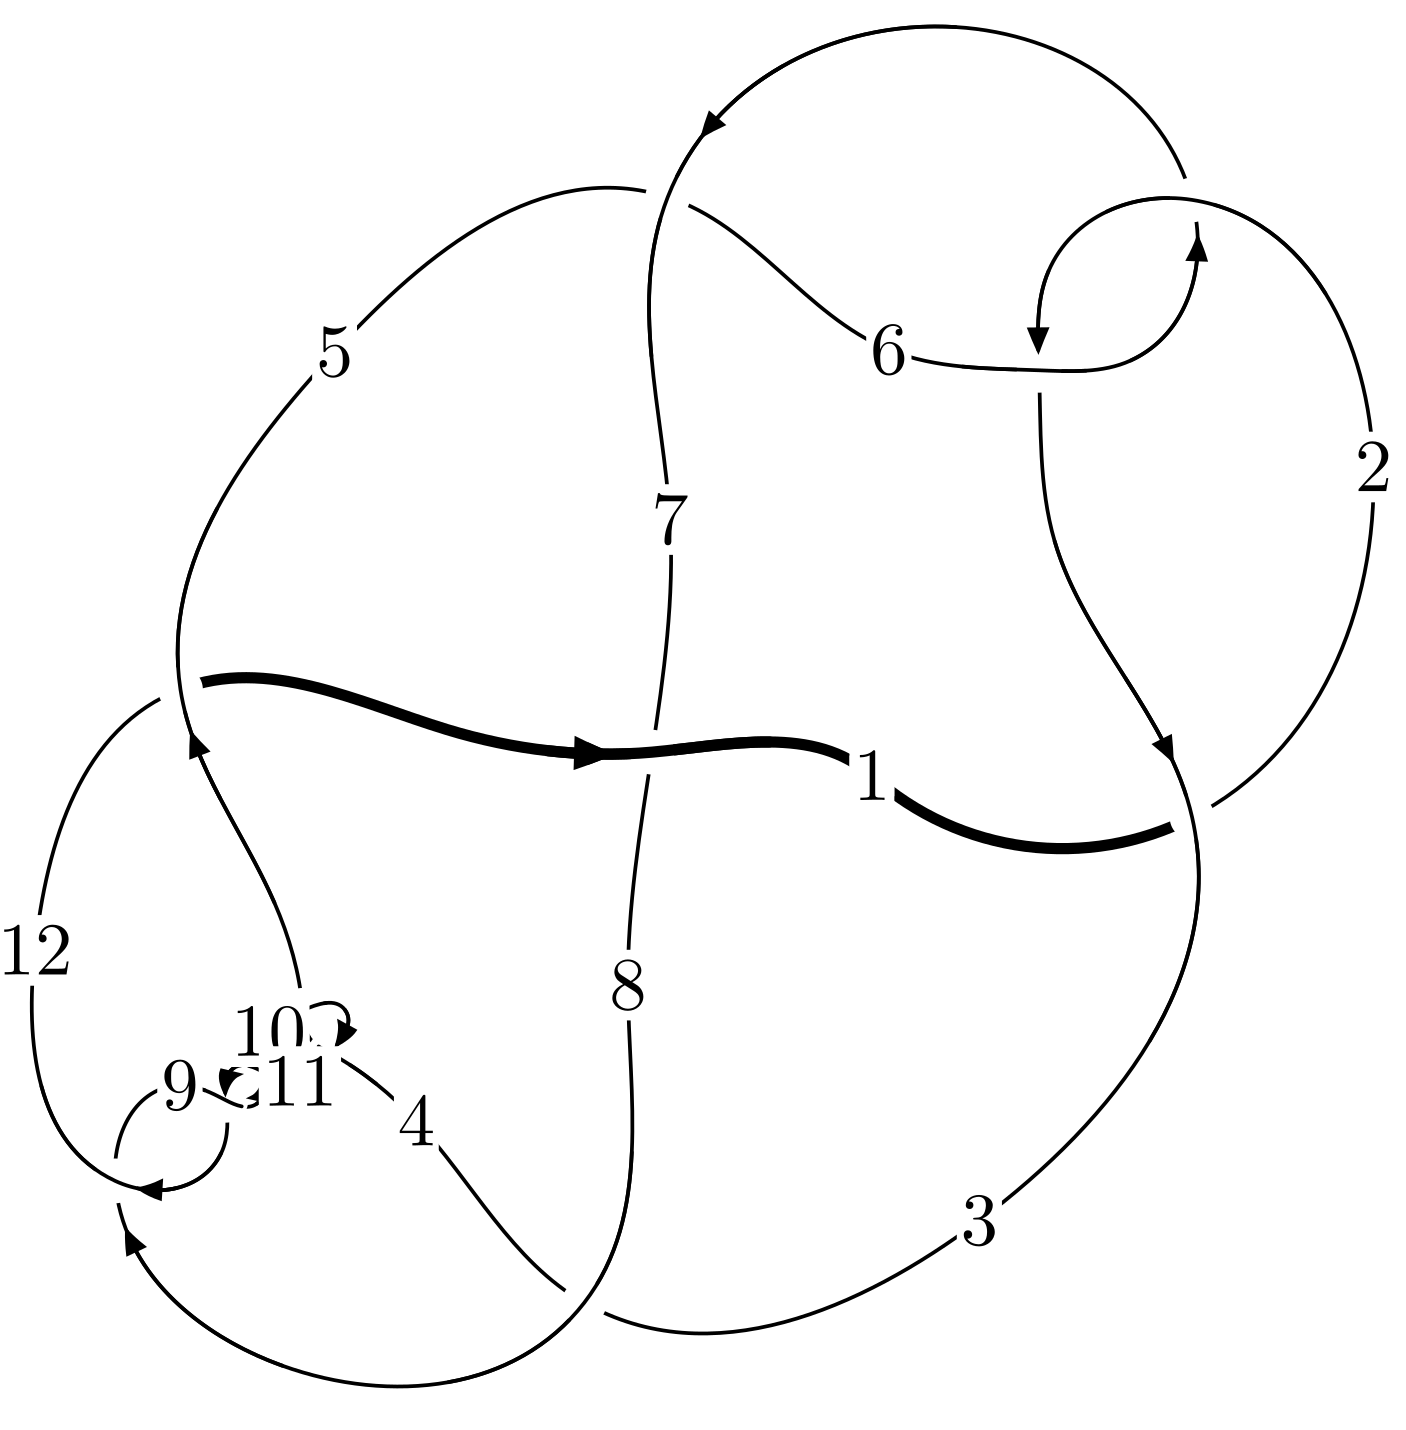
\includegraphics[width=112pt]{../../../GIT/diagram.site/Diagrams/png/1107_12a_0306.png}\\
\ \ \ A knot diagram\footnotemark}&
\allowdisplaybreaks
\textbf{Linearized knot diagam} \\
\cline{2-2}
 &
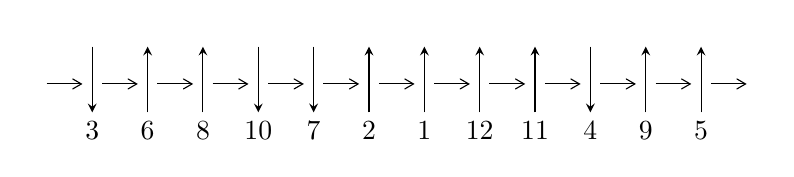
\begin{tikzpicture}[x=20pt, y=17pt]
	% nodes
	\node (C0) at (0, 0) {};
	\node (C1) at (1, 0) {};
	\node (C1U) at (1, +1) {};
	\node (C1D) at (1, -1) {3};

	\node (C2) at (2, 0) {};
	\node (C2U) at (2, +1) {};
	\node (C2D) at (2, -1) {6};

	\node (C3) at (3, 0) {};
	\node (C3U) at (3, +1) {};
	\node (C3D) at (3, -1) {8};

	\node (C4) at (4, 0) {};
	\node (C4U) at (4, +1) {};
	\node (C4D) at (4, -1) {10};

	\node (C5) at (5, 0) {};
	\node (C5U) at (5, +1) {};
	\node (C5D) at (5, -1) {7};

	\node (C6) at (6, 0) {};
	\node (C6U) at (6, +1) {};
	\node (C6D) at (6, -1) {2};

	\node (C7) at (7, 0) {};
	\node (C7U) at (7, +1) {};
	\node (C7D) at (7, -1) {1};

	\node (C8) at (8, 0) {};
	\node (C8U) at (8, +1) {};
	\node (C8D) at (8, -1) {12};

	\node (C9) at (9, 0) {};
	\node (C9U) at (9, +1) {};
	\node (C9D) at (9, -1) {11};

	\node (C10) at (10, 0) {};
	\node (C10U) at (10, +1) {};
	\node (C10D) at (10, -1) {4};

	\node (C11) at (11, 0) {};
	\node (C11U) at (11, +1) {};
	\node (C11D) at (11, -1) {9};

	\node (C12) at (12, 0) {};
	\node (C12U) at (12, +1) {};
	\node (C12D) at (12, -1) {5};
	\node (C13) at (13, 0) {};

	% arrows
	\draw[->,>={angle 60}]
	(C0) edge (C1) (C1) edge (C2) (C2) edge (C3) (C3) edge (C4) (C4) edge (C5) (C5) edge (C6) (C6) edge (C7) (C7) edge (C8) (C8) edge (C9) (C9) edge (C10) (C10) edge (C11) (C11) edge (C12) (C12) edge (C13) ;	\draw[->,>=stealth]
	(C1U) edge (C1D) (C2D) edge (C2U) (C3D) edge (C3U) (C4U) edge (C4D) (C5U) edge (C5D) (C6D) edge (C6U) (C7D) edge (C7U) (C8D) edge (C8U) (C9D) edge (C9U) (C10U) edge (C10D) (C11D) edge (C11U) (C12D) edge (C12U) ;
	\end{tikzpicture} \\
\hhline{~~} \\& 
\textbf{Solving Sequence} \\ \cline{2-2} 
 &
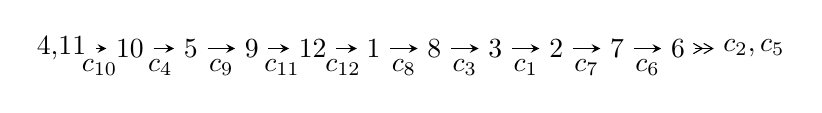
\begin{tikzpicture}[x=22pt, y=7pt]
	% node
	\node (A0) at (-1/8, 0) {4,11};
	\node (A1) at (1, 0) {10};
	\node (A2) at (2, 0) {5};
	\node (A3) at (3, 0) {9};
	\node (A4) at (4, 0) {12};
	\node (A5) at (5, 0) {1};
	\node (A6) at (6, 0) {8};
	\node (A7) at (7, 0) {3};
	\node (A8) at (8, 0) {2};
	\node (A9) at (9, 0) {7};
	\node (A10) at (10, 0) {6};
	\node (C1) at (1/2, -1) {$c_{10}$};
	\node (C2) at (3/2, -1) {$c_{4}$};
	\node (C3) at (5/2, -1) {$c_{9}$};
	\node (C4) at (7/2, -1) {$c_{11}$};
	\node (C5) at (9/2, -1) {$c_{12}$};
	\node (C6) at (11/2, -1) {$c_{8}$};
	\node (C7) at (13/2, -1) {$c_{3}$};
	\node (C8) at (15/2, -1) {$c_{1}$};
	\node (C9) at (17/2, -1) {$c_{7}$};
	\node (C10) at (19/2, -1) {$c_{6}$};
	\node (A11) at (45/4, 0) {$c_{2},c_{5}$};

	% edge
	\draw[->,>=stealth]	
	(A0) edge (A1) (A1) edge (A2) (A2) edge (A3) (A3) edge (A4) (A4) edge (A5) (A5) edge (A6) (A6) edge (A7) (A7) edge (A8) (A8) edge (A9) (A9) edge (A10) ;
	\draw[->>,>={angle 60}]	
	(A10) edge (A11);
\end{tikzpicture} \\ 

\end{tabular} \\

\footnotetext{
The image of knot diagram is generated by the software ``\textbf{Draw programme}" developed by Andrew Bartholomew(\url{http://www.layer8.co.uk/maths/draw/index.htm\#Running-draw}), where we modified some parts for our purpose(\url{https://github.com/CATsTAILs/LinksPainter}).
}\phantom \\ \newline 
\centering \textbf{Ideals for irreducible components\footnotemark of $X_{\text{par}}$} 
 
\begin{align*}
I^u_{1}&=\langle 
u^{66}- u^{65}+\cdots+2 u+1\rangle \\
I^u_{2}&=\langle 
u^7+u^5+2 u^3+u-1\rangle \\
\\
\end{align*}
\raggedright * 2 irreducible components of $\dim_{\mathbb{C}}=0$, with total 73 representations.\\
\footnotetext{All coefficients of polynomials are rational numbers. But the coefficients are sometimes approximated in decimal forms when there is not enough margin.}
\newpage
\renewcommand{\arraystretch}{1}
\centering \section*{I. $I^u_{1}= \langle u^{66}- u^{65}+\cdots+2 u+1 \rangle$}
\flushleft \textbf{(i) Arc colorings}\\
\begin{tabular}{m{7pt} m{180pt} m{7pt} m{180pt} }
\flushright $a_{4}=$&$\begin{pmatrix}0\\u\end{pmatrix}$ \\
\flushright $a_{11}=$&$\begin{pmatrix}1\\0\end{pmatrix}$ \\
\flushright $a_{10}=$&$\begin{pmatrix}1\\- u^2\end{pmatrix}$ \\
\flushright $a_{5}=$&$\begin{pmatrix}- u\\u^3+u\end{pmatrix}$ \\
\flushright $a_{9}=$&$\begin{pmatrix}u^2+1\\- u^2\end{pmatrix}$ \\
\flushright $a_{12}=$&$\begin{pmatrix}u^4+u^2+1\\- u^4\end{pmatrix}$ \\
\flushright $a_{1}=$&$\begin{pmatrix}u^8+u^6+3 u^4+2 u^2+1\\- u^{10}-2 u^8-3 u^6-4 u^4- u^2\end{pmatrix}$ \\
\flushright $a_{8}=$&$\begin{pmatrix}u^6+u^4+2 u^2+1\\- u^6- u^2\end{pmatrix}$ \\
\flushright $a_{3}=$&$\begin{pmatrix}- u^{13}-2 u^{11}-5 u^9-6 u^7-6 u^5-4 u^3- u\\u^{13}+u^{11}+3 u^9+2 u^7+2 u^5+u^3+u\end{pmatrix}$ \\
\flushright $a_{2}=$&$\begin{pmatrix}u^{36}+5 u^{34}+\cdots+u^2+1\\- u^{36}-4 u^{34}+\cdots-12 u^8- u^4\end{pmatrix}$ \\
\flushright $a_{7}=$&$\begin{pmatrix}- u^{24}-3 u^{22}+\cdots+2 u^2+1\\u^{26}+4 u^{24}+\cdots+3 u^6- u^2\end{pmatrix}$ \\
\flushright $a_{6}=$&$\begin{pmatrix}- u^{47}-6 u^{45}+\cdots-4 u^3-2 u\\u^{49}+7 u^{47}+\cdots+2 u^3+u\end{pmatrix}$\\&\end{tabular}
\flushleft \textbf{(ii) Obstruction class $= -1$}\\~\\
\flushleft \textbf{(iii) Cusp Shapes $= 4 u^{64}-4 u^{63}+\cdots+8 u^2+2$}\\~\\
\newpage\renewcommand{\arraystretch}{1}
\flushleft \textbf{(iv) u-Polynomials at the component}\newline \\
\begin{tabular}{m{50pt}|m{274pt}}
Crossings & \hspace{64pt}u-Polynomials at each crossing \\
\hline $$\begin{aligned}c_{1},c_{5}\end{aligned}$$&$\begin{aligned}
&u^{66}+21 u^{65}+\cdots+4 u+1
\end{aligned}$\\
\hline $$\begin{aligned}c_{2},c_{6}\end{aligned}$$&$\begin{aligned}
&u^{66}- u^{65}+\cdots-2 u+1
\end{aligned}$\\
\hline $$\begin{aligned}c_{3},c_{12}\end{aligned}$$&$\begin{aligned}
&u^{66}+6 u^{65}+\cdots+1260 u+392
\end{aligned}$\\
\hline $$\begin{aligned}c_{4},c_{10}\end{aligned}$$&$\begin{aligned}
&u^{66}- u^{65}+\cdots+2 u+1
\end{aligned}$\\
\hline $$\begin{aligned}c_{7}\end{aligned}$$&$\begin{aligned}
&u^{66}+5 u^{65}+\cdots-4 u+37
\end{aligned}$\\
\hline $$\begin{aligned}c_{8},c_{9},c_{11}\end{aligned}$$&$\begin{aligned}
&u^{66}-17 u^{65}+\cdots-4 u+1
\end{aligned}$\\
\hline
\end{tabular}\\~\\
\newpage\renewcommand{\arraystretch}{1}
\flushleft \textbf{(v) Riley Polynomials at the component}\newline \\
\begin{tabular}{m{50pt}|m{274pt}}
Crossings & \hspace{64pt}Riley Polynomials at each crossing \\
\hline $$\begin{aligned}c_{1},c_{5}\end{aligned}$$&$\begin{aligned}
&y^{66}+49 y^{65}+\cdots+76 y+1
\end{aligned}$\\
\hline $$\begin{aligned}c_{2},c_{6}\end{aligned}$$&$\begin{aligned}
&y^{66}+21 y^{65}+\cdots+4 y+1
\end{aligned}$\\
\hline $$\begin{aligned}c_{3},c_{12}\end{aligned}$$&$\begin{aligned}
&y^{66}-42 y^{65}+\cdots+3127376 y+153664
\end{aligned}$\\
\hline $$\begin{aligned}c_{4},c_{10}\end{aligned}$$&$\begin{aligned}
&y^{66}+17 y^{65}+\cdots+4 y+1
\end{aligned}$\\
\hline $$\begin{aligned}c_{7}\end{aligned}$$&$\begin{aligned}
&y^{66}-7 y^{65}+\cdots-10820 y+1369
\end{aligned}$\\
\hline $$\begin{aligned}c_{8},c_{9},c_{11}\end{aligned}$$&$\begin{aligned}
&y^{66}+65 y^{65}+\cdots+4 y+1
\end{aligned}$\\
\hline
\end{tabular}\\~\\
\newpage\flushleft \textbf{(vi) Complex Volumes and Cusp Shapes}
$$\begin{array}{c|c|c}  
\text{Solutions to }I^u_{1}& \I (\text{vol} + \sqrt{-1}CS) & \text{Cusp shape}\\
 \hline 
\begin{aligned}
u &= \phantom{-}0.276142 + 0.973147 I\end{aligned}
 & \phantom{-}4.50590 - 2.85550 I & \phantom{-}12.05805 + 4.41993 I \\ \hline\begin{aligned}
u &= \phantom{-}0.276142 - 0.973147 I\end{aligned}
 & \phantom{-}4.50590 + 2.85550 I & \phantom{-}12.05805 - 4.41993 I \\ \hline\begin{aligned}
u &= -0.311087 + 0.967783 I\end{aligned}
 & \phantom{-}1.20301 + 5.52787 I & \phantom{-}4.00000 - 8.08112 I \\ \hline\begin{aligned}
u &= -0.311087 - 0.967783 I\end{aligned}
 & \phantom{-}1.20301 - 5.52787 I & \phantom{-}4.00000 + 8.08112 I \\ \hline\begin{aligned}
u &= -0.225553 + 0.996987 I\end{aligned}
 & \phantom{-}7.62104 - 4.67869 I & \phantom{-}10.89032 + 2.00709 I \\ \hline\begin{aligned}
u &= -0.225553 - 0.996987 I\end{aligned}
 & \phantom{-}7.62104 + 4.67869 I & \phantom{-}10.89032 - 2.00709 I \\ \hline\begin{aligned}
u &= \phantom{-}0.236153 + 0.997386 I\end{aligned}
 & \phantom{-}8.32399 - 1.19963 I & \phantom{-}12.16015 + 3.25993 I \\ \hline\begin{aligned}
u &= \phantom{-}0.236153 - 0.997386 I\end{aligned}
 & \phantom{-}8.32399 + 1.19963 I & \phantom{-}12.16015 - 3.25993 I \\ \hline\begin{aligned}
u &= \phantom{-}0.304523 + 1.001500 I\end{aligned}
 & \phantom{-}7.92106 - 4.82325 I & \phantom{-}11.07978 + 4.36296 I \\ \hline\begin{aligned}
u &= \phantom{-}0.304523 - 1.001500 I\end{aligned}
 & \phantom{-}7.92106 + 4.82325 I & \phantom{-}11.07978 - 4.36296 I \\ \hline\begin{aligned}
u &= -0.312943 + 1.002150 I\end{aligned}
 & \phantom{-}7.10672 + 10.70210 I & \phantom{-}9.44810 - 9.41252 I \\ \hline\begin{aligned}
u &= -0.312943 - 1.002150 I\end{aligned}
 & \phantom{-}7.10672 - 10.70210 I & \phantom{-}9.44810 + 9.41252 I \\ \hline\begin{aligned}
u &= \phantom{-}0.456777 + 0.785683 I\end{aligned}
 & \phantom{-}1.23819 - 6.54922 I & \phantom{-}4.17677 + 9.67765 I \\ \hline\begin{aligned}
u &= \phantom{-}0.456777 - 0.785683 I\end{aligned}
 & \phantom{-}1.23819 + 6.54922 I & \phantom{-}4.17677 - 9.67765 I \\ \hline\begin{aligned}
u &= -0.397793 + 0.800537 I\end{aligned}
 & \phantom{-}1.82221 + 1.25981 I & \phantom{-}6.09781 - 4.41931 I \\ \hline\begin{aligned}
u &= -0.397793 - 0.800537 I\end{aligned}
 & \phantom{-}1.82221 - 1.25981 I & \phantom{-}6.09781 + 4.41931 I \\ \hline\begin{aligned}
u &= \phantom{-}0.784027 + 0.781220 I\end{aligned}
 & \phantom{-}1.10586 - 5.81643 I & \phantom{-0.000000 } 0 \\ \hline\begin{aligned}
u &= \phantom{-}0.784027 - 0.781220 I\end{aligned}
 & \phantom{-}1.10586 + 5.81643 I & \phantom{-0.000000 } 0 \\ \hline\begin{aligned}
u &= -0.023490 + 0.865695 I\end{aligned}
 & \phantom{-}3.89741 + 2.71211 I & \phantom{-}12.15997 - 3.32953 I \\ \hline\begin{aligned}
u &= -0.023490 - 0.865695 I\end{aligned}
 & \phantom{-}3.89741 - 2.71211 I & \phantom{-}12.15997 + 3.32953 I \\ \hline\begin{aligned}
u &= -0.836827 + 0.807352 I\end{aligned}
 & -2.60329 - 1.13595 I & \phantom{-0.000000 } 0 \\ \hline\begin{aligned}
u &= -0.836827 - 0.807352 I\end{aligned}
 & -2.60329 + 1.13595 I & \phantom{-0.000000 } 0 \\ \hline\begin{aligned}
u &= -0.858606 + 0.795301 I\end{aligned}
 & \phantom{-}0.37310 - 3.30299 I & \phantom{-0.000000 } 0 \\ \hline\begin{aligned}
u &= -0.858606 - 0.795301 I\end{aligned}
 & \phantom{-}0.37310 + 3.30299 I & \phantom{-0.000000 } 0 \\ \hline\begin{aligned}
u &= \phantom{-}0.863434 + 0.797395 I\end{aligned}
 & -0.53580 + 9.14737 I & \phantom{-0.000000 } 0 \\ \hline\begin{aligned}
u &= \phantom{-}0.863434 - 0.797395 I\end{aligned}
 & -0.53580 - 9.14737 I & \phantom{-0.000000 } 0 \\ \hline\begin{aligned}
u &= \phantom{-}0.827585 + 0.837312 I\end{aligned}
 & -4.93871 - 2.14028 I & \phantom{-0.000000 } 0 \\ \hline\begin{aligned}
u &= \phantom{-}0.827585 - 0.837312 I\end{aligned}
 & -4.93871 + 2.14028 I & \phantom{-0.000000 } 0 \\ \hline\begin{aligned}
u &= \phantom{-}0.854921 + 0.812716 I\end{aligned}
 & -6.26873 + 3.63660 I & \phantom{-0.000000 } 0 \\ \hline\begin{aligned}
u &= \phantom{-}0.854921 - 0.812716 I\end{aligned}
 & -6.26873 - 3.63660 I & \phantom{-0.000000 } 0\\
 \hline 
 \end{array}$$\newpage$$\begin{array}{c|c|c}  
\text{Solutions to }I^u_{1}& \I (\text{vol} + \sqrt{-1}CS) & \text{Cusp shape}\\
 \hline 
\begin{aligned}
u &= \phantom{-}0.827211 + 0.875814 I\end{aligned}
 & -5.15023 - 2.33627 I & \phantom{-0.000000 } 0 \\ \hline\begin{aligned}
u &= \phantom{-}0.827211 - 0.875814 I\end{aligned}
 & -5.15023 + 2.33627 I & \phantom{-0.000000 } 0 \\ \hline\begin{aligned}
u &= -0.845186 + 0.880793 I\end{aligned}
 & -6.18098 - 2.57775 I & \phantom{-0.000000 } 0 \\ \hline\begin{aligned}
u &= -0.845186 - 0.880793 I\end{aligned}
 & -6.18098 + 2.57775 I & \phantom{-0.000000 } 0 \\ \hline\begin{aligned}
u &= \phantom{-}0.459757 + 0.623778 I\end{aligned}
 & -3.05863 - 1.75367 I & -4.05356 + 5.04373 I \\ \hline\begin{aligned}
u &= \phantom{-}0.459757 - 0.623778 I\end{aligned}
 & -3.05863 + 1.75367 I & -4.05356 - 5.04373 I \\ \hline\begin{aligned}
u &= \phantom{-}0.815789 + 0.918639 I\end{aligned}
 & -5.01899 - 3.79645 I & \phantom{-0.000000 } 0 \\ \hline\begin{aligned}
u &= \phantom{-}0.815789 - 0.918639 I\end{aligned}
 & -5.01899 + 3.79645 I & \phantom{-0.000000 } 0 \\ \hline\begin{aligned}
u &= -0.761181 + 0.966217 I\end{aligned}
 & \phantom{-}2.20192 + 5.87663 I & \phantom{-0.000000 } 0 \\ \hline\begin{aligned}
u &= -0.761181 - 0.966217 I\end{aligned}
 & \phantom{-}2.20192 - 5.87663 I & \phantom{-0.000000 } 0 \\ \hline\begin{aligned}
u &= -0.837522 + 0.902945 I\end{aligned}
 & -9.94428 + 3.11601 I & \phantom{-0.000000 } 0 \\ \hline\begin{aligned}
u &= -0.837522 - 0.902945 I\end{aligned}
 & -9.94428 - 3.11601 I & \phantom{-0.000000 } 0 \\ \hline\begin{aligned}
u &= \phantom{-}0.791445 + 0.947693 I\end{aligned}
 & -4.59364 - 3.91730 I & \phantom{-0.000000 } 0 \\ \hline\begin{aligned}
u &= \phantom{-}0.791445 - 0.947693 I\end{aligned}
 & -4.59364 + 3.91730 I & \phantom{-0.000000 } 0 \\ \hline\begin{aligned}
u &= -0.830031 + 0.923795 I\end{aligned}
 & -6.04701 + 8.80946 I & \phantom{-0.000000 } 0 \\ \hline\begin{aligned}
u &= -0.830031 - 0.923795 I\end{aligned}
 & -6.04701 - 8.80946 I & \phantom{-0.000000 } 0 \\ \hline\begin{aligned}
u &= -0.787054 + 0.967827 I\end{aligned}
 & -2.10788 + 7.20390 I & \phantom{-0.000000 } 0 \\ \hline\begin{aligned}
u &= -0.787054 - 0.967827 I\end{aligned}
 & -2.10788 - 7.20390 I & \phantom{-0.000000 } 0 \\ \hline\begin{aligned}
u &= \phantom{-}0.798774 + 0.972679 I\end{aligned}
 & -5.77098 - 9.79547 I & \phantom{-0.000000 } 0 \\ \hline\begin{aligned}
u &= \phantom{-}0.798774 - 0.972679 I\end{aligned}
 & -5.77098 + 9.79547 I & \phantom{-0.000000 } 0 \\ \hline\begin{aligned}
u &= -0.792645 + 0.983270 I\end{aligned}
 & \phantom{-}0.95662 + 9.45046 I & \phantom{-0.000000 } 0 \\ \hline\begin{aligned}
u &= -0.792645 - 0.983270 I\end{aligned}
 & \phantom{-}0.95662 - 9.45046 I & \phantom{-0.000000 } 0 \\ \hline\begin{aligned}
u &= \phantom{-}0.795929 + 0.984558 I\end{aligned}
 & \phantom{-}0.0466 - 15.3200 I & \phantom{-0.000000 } 0 \\ \hline\begin{aligned}
u &= \phantom{-}0.795929 - 0.984558 I\end{aligned}
 & \phantom{-}0.0466 + 15.3200 I & \phantom{-0.000000 } 0 \\ \hline\begin{aligned}
u &= -0.223454 + 0.622794 I\end{aligned}
 & \phantom{-}0.329896 + 0.949161 I & \phantom{-}5.93547 - 7.10571 I \\ \hline\begin{aligned}
u &= -0.223454 - 0.622794 I\end{aligned}
 & \phantom{-}0.329896 - 0.949161 I & \phantom{-}5.93547 + 7.10571 I \\ \hline\begin{aligned}
u &= \phantom{-}0.487684 + 0.434861 I\end{aligned}
 & \phantom{-}0.22976 + 2.99529 I & \phantom{-}0.08554 - 2.50316 I \\ \hline\begin{aligned}
u &= \phantom{-}0.487684 - 0.434861 I\end{aligned}
 & \phantom{-}0.22976 - 2.99529 I & \phantom{-}0.08554 + 2.50316 I \\ \hline\begin{aligned}
u &= -0.643478 + 0.086667 I\end{aligned}
 & \phantom{-}4.24877 - 7.37536 I & \phantom{-}3.63430 + 5.60307 I \\ \hline\begin{aligned}
u &= -0.643478 - 0.086667 I\end{aligned}
 & \phantom{-}4.24877 + 7.37536 I & \phantom{-}3.63430 - 5.60307 I\\
 \hline 
 \end{array}$$\newpage$$\begin{array}{c|c|c}  
\text{Solutions to }I^u_{1}& \I (\text{vol} + \sqrt{-1}CS) & \text{Cusp shape}\\
 \hline 
\begin{aligned}
u &= \phantom{-}0.638810 + 0.068850 I\end{aligned}
 & \phantom{-}5.02009 + 1.56359 I & \phantom{-}5.22655 - 0.46859 I \\ \hline\begin{aligned}
u &= \phantom{-}0.638810 - 0.068850 I\end{aligned}
 & \phantom{-}5.02009 - 1.56359 I & \phantom{-}5.22655 + 0.46859 I \\ \hline\begin{aligned}
u &= -0.565065 + 0.112376 I\end{aligned}
 & -1.37963 - 2.39285 I & -2.15770 + 3.99262 I \\ \hline\begin{aligned}
u &= -0.565065 - 0.112376 I\end{aligned}
 & -1.37963 + 2.39285 I & -2.15770 - 3.99262 I \\ \hline\begin{aligned}
u &= -0.467047 + 0.336383 I\end{aligned}
 & \phantom{-}0.51184 + 1.97273 I & \phantom{-}0.43404 - 3.18104 I \\ \hline\begin{aligned}
u &= -0.467047 - 0.336383 I\end{aligned}
 & \phantom{-}0.51184 - 1.97273 I & \phantom{-}0.43404 + 3.18104 I\\
 \hline 
 \end{array}$$\newpage\newpage\renewcommand{\arraystretch}{1}
\centering \section*{II. $I^u_{2}= \langle u^7+u^5+2 u^3+u-1 \rangle$}
\flushleft \textbf{(i) Arc colorings}\\
\begin{tabular}{m{7pt} m{180pt} m{7pt} m{180pt} }
\flushright $a_{4}=$&$\begin{pmatrix}0\\u\end{pmatrix}$ \\
\flushright $a_{11}=$&$\begin{pmatrix}1\\0\end{pmatrix}$ \\
\flushright $a_{10}=$&$\begin{pmatrix}1\\- u^2\end{pmatrix}$ \\
\flushright $a_{5}=$&$\begin{pmatrix}- u\\u^3+u\end{pmatrix}$ \\
\flushright $a_{9}=$&$\begin{pmatrix}u^2+1\\- u^2\end{pmatrix}$ \\
\flushright $a_{12}=$&$\begin{pmatrix}u^4+u^2+1\\- u^4\end{pmatrix}$ \\
\flushright $a_{1}=$&$\begin{pmatrix}u^4+u^2+u+1\\- u^4- u^3- u\end{pmatrix}$ \\
\flushright $a_{8}=$&$\begin{pmatrix}u^6+u^4+2 u^2+1\\- u^6- u^2\end{pmatrix}$ \\
\flushright $a_{3}=$&$\begin{pmatrix}- u^6- u^4-2 u^2-1\\u^6+u^2+u\end{pmatrix}$ \\
\flushright $a_{2}=$&$\begin{pmatrix}u^4+u^2+1\\- u^6-2 u^4- u^2\end{pmatrix}$ \\
\flushright $a_{7}=$&$\begin{pmatrix}u^3\\- u^5- u^3+u\end{pmatrix}$ \\
\flushright $a_{6}=$&$\begin{pmatrix}- u^5- u\\-2 u^3+1\end{pmatrix}$\\&\end{tabular}
\flushleft \textbf{(ii) Obstruction class $= -1$}\\~\\
\flushleft \textbf{(iii) Cusp Shapes $= 6$}\\~\\
\newpage\renewcommand{\arraystretch}{1}
\flushleft \textbf{(iv) u-Polynomials at the component}\newline \\
\begin{tabular}{m{50pt}|m{274pt}}
Crossings & \hspace{64pt}u-Polynomials at each crossing \\
\hline $$\begin{aligned}c_{1},c_{5}\end{aligned}$$&$\begin{aligned}
&u^7+2 u^6+5 u^5+6 u^4+6 u^3+4 u^2+u-1
\end{aligned}$\\
\hline $$\begin{aligned}c_{2},c_{4},c_{6}\\c_{10}\end{aligned}$$&$\begin{aligned}
&u^7+u^5+2 u^3+u-1
\end{aligned}$\\
\hline $$\begin{aligned}c_{3},c_{12}\end{aligned}$$&$\begin{aligned}
&(u-1)^7
\end{aligned}$\\
\hline $$\begin{aligned}c_{7}\end{aligned}$$&$\begin{aligned}
&u^7-3 u^5-2 u^4+8 u^3+2 u^2- u-3
\end{aligned}$\\
\hline $$\begin{aligned}c_{8},c_{9},c_{11}\end{aligned}$$&$\begin{aligned}
&u^7-2 u^6+5 u^5-6 u^4+6 u^3-4 u^2+u+1
\end{aligned}$\\
\hline
\end{tabular}\\~\\
\newpage\renewcommand{\arraystretch}{1}
\flushleft \textbf{(v) Riley Polynomials at the component}\newline \\
\begin{tabular}{m{50pt}|m{274pt}}
Crossings & \hspace{64pt}Riley Polynomials at each crossing \\
\hline $$\begin{aligned}c_{1},c_{5},c_{8}\\c_{9},c_{11}\end{aligned}$$&$\begin{aligned}
&y^7+6 y^6+13 y^5+10 y^4+2 y^3+8 y^2+9 y-1
\end{aligned}$\\
\hline $$\begin{aligned}c_{2},c_{4},c_{6}\\c_{10}\end{aligned}$$&$\begin{aligned}
&y^7+2 y^6+5 y^5+6 y^4+6 y^3+4 y^2+y-1
\end{aligned}$\\
\hline $$\begin{aligned}c_{3},c_{12}\end{aligned}$$&$\begin{aligned}
&(y-1)^7
\end{aligned}$\\
\hline $$\begin{aligned}c_{7}\end{aligned}$$&$\begin{aligned}
&y^7-6 y^6+25 y^5-54 y^4+78 y^3-32 y^2+13 y-9
\end{aligned}$\\
\hline
\end{tabular}\\~\\
\newpage\flushleft \textbf{(vi) Complex Volumes and Cusp Shapes}
$$\begin{array}{c|c|c}  
\text{Solutions to }I^u_{2}& \I (\text{vol} + \sqrt{-1}CS) & \text{Cusp shape}\\
 \hline 
\begin{aligned}
u &= -0.237779 + 0.943997 I\end{aligned}
 & \phantom{-}1.64493\phantom{ +0.000000I} & \phantom{-}6.00000\phantom{ +0.000000I} \\ \hline\begin{aligned}
u &= -0.237779 - 0.943997 I\end{aligned}
 & \phantom{-}1.64493\phantom{ +0.000000I} & \phantom{-}6.00000\phantom{ +0.000000I} \\ \hline\begin{aligned}
u &= -0.799839 + 0.781167 I\end{aligned}
 & \phantom{-}1.64493\phantom{ +0.000000I} & \phantom{-}6.00000\phantom{ +0.000000I} \\ \hline\begin{aligned}
u &= -0.799839 - 0.781167 I\end{aligned}
 & \phantom{-}1.64493\phantom{ +0.000000I} & \phantom{-}6.00000\phantom{ +0.000000I} \\ \hline\begin{aligned}
u &= \phantom{-}0.755347 + 0.961681 I\end{aligned}
 & \phantom{-}1.64493\phantom{ +0.000000I} & \phantom{-}6.00000\phantom{ +0.000000I} \\ \hline\begin{aligned}
u &= \phantom{-}0.755347 - 0.961681 I\end{aligned}
 & \phantom{-}1.64493\phantom{ +0.000000I} & \phantom{-}6.00000\phantom{ +0.000000I} \\ \hline\begin{aligned}
u &= \phantom{-}0.564540\phantom{ +0.000000I}\end{aligned}
 & \phantom{-}1.64493\phantom{ +0.000000I} & \phantom{-}6.00000\phantom{ +0.000000I}\\
 \hline 
 \end{array}$$\newpage
\newpage\renewcommand{\arraystretch}{1}
\centering \section*{ III. u-Polynomials}
\begin{tabular}{m{50pt}|m{274pt}}
Crossings & \hspace{64pt}u-Polynomials at each crossing \\
\hline $$\begin{aligned}c_{1},c_{5}\end{aligned}$$&$\begin{aligned}
&(u^7+2 u^6+\cdots+u-1)(u^{66}+21 u^{65}+\cdots+4 u+1)
\end{aligned}$\\
\hline $$\begin{aligned}c_{2},c_{6}\end{aligned}$$&$\begin{aligned}
&(u^7+u^5+2 u^3+u-1)(u^{66}- u^{65}+\cdots-2 u+1)
\end{aligned}$\\
\hline $$\begin{aligned}c_{3},c_{12}\end{aligned}$$&$\begin{aligned}
&((u-1)^7)(u^{66}+6 u^{65}+\cdots+1260 u+392)
\end{aligned}$\\
\hline $$\begin{aligned}c_{4},c_{10}\end{aligned}$$&$\begin{aligned}
&(u^7+u^5+2 u^3+u-1)(u^{66}- u^{65}+\cdots+2 u+1)
\end{aligned}$\\
\hline $$\begin{aligned}c_{7}\end{aligned}$$&$\begin{aligned}
&(u^7-3 u^5-2 u^4+8 u^3+2 u^2- u-3)(u^{66}+5 u^{65}+\cdots-4 u+37)
\end{aligned}$\\
\hline $$\begin{aligned}c_{8},c_{9},c_{11}\end{aligned}$$&$\begin{aligned}
&(u^7-2 u^6+\cdots+u+1)(u^{66}-17 u^{65}+\cdots-4 u+1)
\end{aligned}$\\
\hline
\end{tabular}\newpage\renewcommand{\arraystretch}{1}
\centering \section*{ IV. Riley Polynomials}
\begin{tabular}{m{50pt}|m{274pt}}
Crossings & \hspace{64pt}Riley Polynomials at each crossing \\
\hline $$\begin{aligned}c_{1},c_{5}\end{aligned}$$&$\begin{aligned}
&(y^7+6 y^6+13 y^5+10 y^4+2 y^3+8 y^2+9 y-1)\\
&\cdot(y^{66}+49 y^{65}+\cdots+76 y+1)
\end{aligned}$\\
\hline $$\begin{aligned}c_{2},c_{6}\end{aligned}$$&$\begin{aligned}
&(y^7+2 y^6+\cdots+y-1)(y^{66}+21 y^{65}+\cdots+4 y+1)
\end{aligned}$\\
\hline $$\begin{aligned}c_{3},c_{12}\end{aligned}$$&$\begin{aligned}
&((y-1)^7)(y^{66}-42 y^{65}+\cdots+3127376 y+153664)
\end{aligned}$\\
\hline $$\begin{aligned}c_{4},c_{10}\end{aligned}$$&$\begin{aligned}
&(y^7+2 y^6+\cdots+y-1)(y^{66}+17 y^{65}+\cdots+4 y+1)
\end{aligned}$\\
\hline $$\begin{aligned}c_{7}\end{aligned}$$&$\begin{aligned}
&(y^7-6 y^6+25 y^5-54 y^4+78 y^3-32 y^2+13 y-9)\\
&\cdot(y^{66}-7 y^{65}+\cdots-10820 y+1369)
\end{aligned}$\\
\hline $$\begin{aligned}c_{8},c_{9},c_{11}\end{aligned}$$&$\begin{aligned}
&(y^7+6 y^6+13 y^5+10 y^4+2 y^3+8 y^2+9 y-1)\\
&\cdot(y^{66}+65 y^{65}+\cdots+4 y+1)
\end{aligned}$\\
\hline
\end{tabular}
\vskip 2pc
\end{document}